\begin{theorem} Для простейшего симметричного блуждания верно, что
$
P\brackets{\overline{\lim\limits_{n \to \infty}}\frac{|S_n|}{\sqrt{2n\cdot lnlnn}} = 1} = 1
$\\
\end{theorem}
\vspace{-4ex}
\begin{figure}[h] \begin{minipage}[h]{0.5\linewidth}
    \center{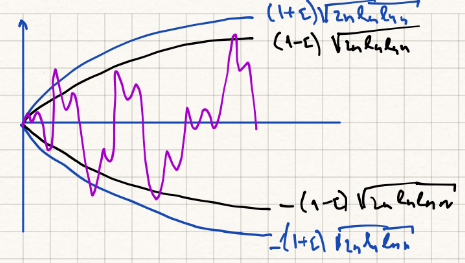
\includegraphics[width=1\textwidth]{images/tv4.png}}
\end{minipage}
\begin{minipage}[h]{0.5\linewidth}
    То есть для почти всех траекторий $S_n$ конечное количество раз больше единицы и бесконечное количество раз меньше единицы. На рисунке это значит, что траекторий пересекает синюю кривую конечное число раз, а черную бесконечное число раз.
\end{minipage}
\end{figure}
% 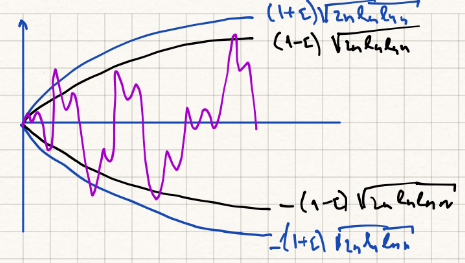
\includegraphics[width=0.3\textwidth]{images/tv4.png}
% То есть для почти всех траекторий $S_n$ конечное количество раз больше единицы и бесконечное количество раз меньше единицы. На рисунке это значит, что траекторий пересекает синюю кривую конечное число раз, а черную бесконечное число раз.
\begin{definition} Пусть $A_1\ A_2, \ldots \in \F$, тогда событие $A_n \text{ б.ч.} = \bigcap\limits_{n = 1}^\infty\bigcup\limits_{k \geqslant n}^\infty A_k$ (бесконечно часто), то есть множество тех элементарных исходов, которые попадают в бесконечное множество событий.
\end{definition} 
\begin{theorem}\textbf{Лемма Бореля-Кантелли}
\begin{enumerate}
    \item Если $\sum\limits_{n = 1}^\infty P(A_n) < \infty$, то $P(A_n \text{ б.ч.}) = 0$
    \item Если $A_1, A_2, \ldots$ независимы и $\sum\limits_{n = 1}^\infty P(A_n) = \infty$, то $P(A_n \text{б.ч.}) = 1$
\end{enumerate}
\end{theorem}

\begin{proof}
   1. $
    P(A_n \text{ б.ч.}) = P\brackets{\bigcap\limits_{n \in \N}\bigcup\limits_{m \geqslant n}A_m} = \lim\limits_{n \to \infty} P\brackets{\bigcup\limits_{m \geqslant n}A_m} \leqslant \lim\limits_{n \to \infty} \sum\limits_{m \geqslant n} P(A_m) = 0
    $\\
    Где второе равенство по теореме о непрерывности меры \\
    2.
    $
         P(A_n \text{ б.ч.}) = P\brackets{\bigcap\limits_{n \in \N}\bigcup\limits_{m \geqslant n}A_m} =  1 - P\brackets{\bigcup\limits_{n \in \N}\bigcap\limits_{m \geqslant n}\overline{A_m}} = 1 - \lim\limits_{n \to \infty} P\brackets{\bigcap\limits_{m \geqslant n} \overline{A_m}} = 1 - \lim\limits_{n \to \infty} \prod\limits_{m \geqslant n} P\brackets{\overline{A_m}} =$ \\
         $= 1 - \lim\limits_{n \to \infty} \exp\brackets{\sum\limits_{m \geqslant n} ln\brackets{1 - P(A_m)}} \geqslant 1 - \lim\limits_{n \to \infty} \exp\brackets{-\sum\limits_{m \geqslant n} P(A_m)} = 1
   $\\
    Где неравенство за счет ряда Тейлора для логарифма.
\end{proof}
\textbf{Пример применения леммы Бореля–Кантелли}

Пусть $\xi_1, \xi_2, \ldots \sim Exp(1)$ и независимы. Доказать, что $P\brackets{\overline{\lim\limits_{n \to\infty}} \frac{\xi_n}{ln \: n} = 1} = 1$
\begin{enumerate}
    \item Докажем, что $P\brackets{\overline{\lim\limits_{n \to\infty}} \frac{\xi_n}{ln \: n} \geqslant 1} = 1$
    \begin{multline*}
        P\brackets{\overline{\lim\limits_{n \to\infty}} \frac{\xi_n}{ln \: n} \geqslant 1} = 1 \Longleftrightarrow P\brackets{\forall \eps > 0 \ \  \forall k \ \exists n \geqslant k: \: \frac{\xi_n}{ln \: n} \geqslant 1 - \eps} = 1 \Longleftrightarrow \\
        \Longleftrightarrow P\brackets{\forall m \in \N \ \ \forall k \ \exists n \geqslant k: \: \frac{\xi_n}{ln \: n} \geqslant 1 - \frac{1}{m}} = 1 \Longleftrightarrow P\brackets{\bigcap\limits_{m = 1}^\infty \bigcap\limits_{k = 1}^\infty \bigcup\limits_{n = k}^\infty \: \frac{\xi_n}{ln \: n} \geqslant 1 - \frac{1}{m}} = 1 \Longleftrightarrow \\
        \Longleftrightarrow \lim\limits_{m \to \infty} P\brackets{\brackets{\frac{\xi_n}{ln \: n} \geqslant 1 - \frac{1}{m}} \text{ б.ч.}} = 1
    \end{multline*}
    $
    \sum\limits_{n = 1}^\infty P\brackets{\frac{\xi_n}{ln \: n} \geqslant 1 - \frac{1}{m}} = \sum\limits_{n = 1}^\infty P\brackets{\xi_n \geqslant \brackets{1 - \frac{1}{m}}ln \: n} = \sum\limits_{n = 1}^\infty \Big (
    \int\limits_{ln \ n (1 - \frac{1}{m})}^{+\infty} e^{-x} dx \Big ) = $\\ $ \sum\limits_{n = 1}^\infty \brackets{e^{-\brackets{1 - \frac{1}{m}}ln\:n}} = \sum\limits_{n = 1}^\infty \brackets{n^{-1 + \frac{1}{m}}} = \infty
    $
    
    Тогда по лемме Бореля-Кантелли событие происходит бесконечно часто, а значит первая часть утверждения доказана.
    
    \item Докажем, что $P\brackets{\overline{\lim\limits_{n \to\infty}} \frac{\xi_n}{ln \: n} \leqslant 1} = 1$
    \begin{multline*}
        P\brackets{\overline{\lim\limits_{n \to\infty}} \frac{\xi_n}{ln \: n} \leqslant 1} = 1 \Longleftrightarrow P\brackets{\forall \eps > 0 \ \ \exists k \ \forall n \geqslant k: \: \frac{\xi_n}{ln \: n} \leqslant 1 + \eps} = 1 \Longleftrightarrow \\
        \Longleftrightarrow P\brackets{\overline{\exists m \in \N \ \  \forall k \ \exists n \geqslant k: \: \frac{\xi_n}{ln \: n} > 1 + \frac{1}{m}}} = 1 \Longleftrightarrow P\brackets{\bigcup\limits_{m = 1}^\infty \bigcap\limits_{k = 1}^\infty \bigcup\limits_{n = k}^\infty \: \frac{\xi_n}{ln \: n} > 1 + \frac{1}{m}} = 0 \Longleftrightarrow \\
        \Longleftrightarrow \lim\limits_{m \to \infty} P\brackets{\brackets{\frac{\xi_n}{ln \: n} > 1 + \frac{1}{m}} \text{ б.ч.}} = 0
    \end{multline*}
    $
    \sum\limits_{n = 1}^\infty P\brackets{\frac{\xi_n}{ln \: n} > 1 + \frac{1}{m}} = \sum\limits_{n = 1}^\infty P\brackets{\xi_n > \brackets{1 + \frac{1}{m}}ln \: n} = \sum\limits_{n = 1}^\infty \Big (
    \int\limits_{ln \ n (1 + \frac{1}{m})}^{+\infty} e^{-x} dx \Big ) =$ \\ $= \sum\limits_{n = 1}^\infty \brackets{e^{-\brackets{1 + \frac{1}{m}}ln\:n}} = \sum\limits_{n = 1}^\infty \brackets{n^{-1 - \frac{1}{m}}} < \infty
    $
    
    Тогда по лемме Бореля-Кантелли вероятность отрицания события равна нулю, а значит вероятность самого события единица, то есть вторая часть (как и все утверждение) доказаны.
\end{enumerate}